% !TEX root = main.tex
\section{概要}

図 \ref{fig:robot1}, \ref{fig:robot2} に示す 4 リンク 2 軸ロボット実験装置は,
ギアを介して軸 $P_1$, $P_5$ に取り付けられた 2 つのモータにより手先の位置 $P_3$ を目標位置に追従させることを
目的とした実験装置である.
このことを実現するためには,手先位置からモータの回転角度を求める逆動力学とモータの回転角度から手先位置を求める
順動力学を理解する必要がある.

\begin{figure}[htbp]
    \centering
    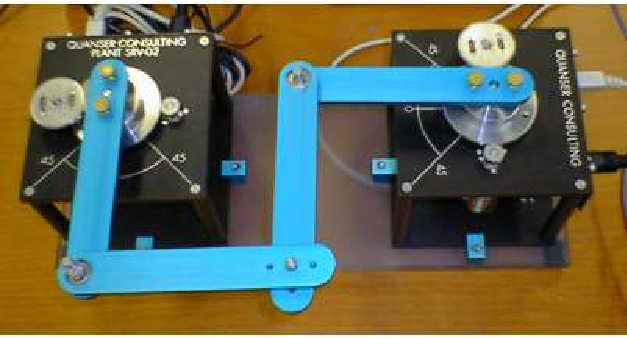
\includegraphics[width=0.6\textwidth]{figure/robot_fig1.pdf}
    \caption{4リンク2軸ロボット実験装置(型番:55023)}
    \label{fig:robot1}
\end{figure}

\begin{figure}[htbp]
    \centering
    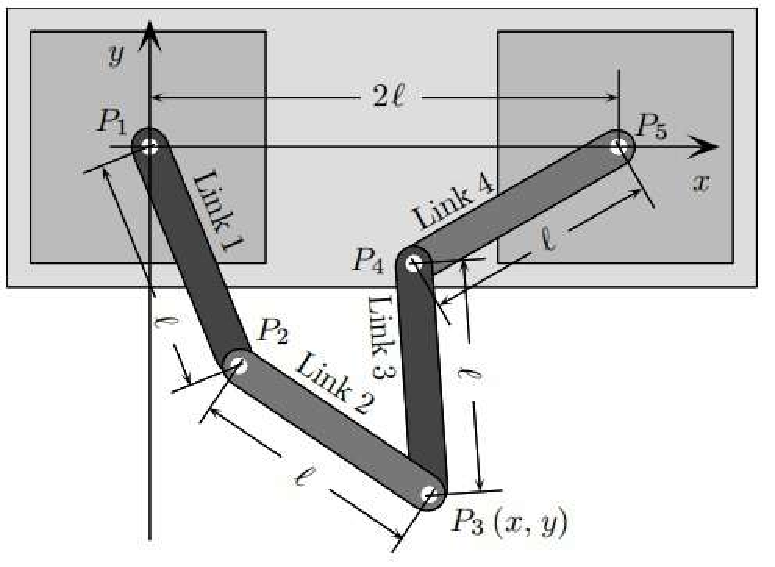
\includegraphics[width=0.6\textwidth]{figure/robot_fig2.pdf}
    \caption{4つリンクの関係}
    \label{fig:robot2}
\end{figure}
